
\documentclass[a4paper]{article}
\pagestyle{plain}
\usepackage[utf8]{inputenc}
\usepackage[english,ukrainian]{babel}
\usepackage[pdftex]{graphicx}
\usepackage{amsmath,amssymb}

\paperwidth=210mm
\paperheight=297mm

\hoffset=0.0mm 		% By default offset from paper edge is 1 inch, this will set it to 25mm
\voffset=-5.4mm		% By default offset from paper edge is 1 inch, this will set it to 20mm

\oddsidemargin=0mm	% This will add nothing to hoffset
\evensidemargin=0mm	% This will add nothing to hoffset
\topmargin=0mm
\headheight=0mm
\headsep=0mm

\textwidth=170mm
\textheight=237mm

\begin{document}

\title{Фотометричний парадокс, або парадокс Ольберса}
\author{\textsl{Ю.\,А.~Грищенко$^{1}$}}
\date{\vspace*{-6ex}}
\maketitle
\begin{center} 
{\small $^{1}$Група К-29, курс 2, факультет кібернетики\\
{\tt yu.hrysh@gmail.com}}
\end{center}

Чому небо вночі темне, а вдень світле? Ми знаємо, що в небі над нами безліч зірок, які принципово нічим не відрізняються від нашого Сонця. Дійсно, відстань між Землею та Сонцем набагто менша за відстань між нами та будь-якою іншою зіркою, але ж у вакуумі світло не розсіюється. Якби можна було взяти Сонце і перенсти його на вдвічі більшу відстань, то на нас би падало в чотири рази менше фотонів, проте воно би займало в чотири рази менше місця на небі, отже яскравість зірки в результаті цього не змінилася би. \cite{relativityFAQ}

Зробимо такі припущення: Всесвіт нескінченний, статичний, у ньому нескінченна кількість зірок, розподілених з постійною щільністю. Тоді будь-який промінь зору має закінчюватися зорею. Аналогом для цього є густий ліс: людина, яка опиниласия у такому середовищі, виявлятиме себе оточеною "стіною" з віддалених дерев, куди би вона не подивилась.

У такому випадку нічне небо повинно бути заповнене яскравим світлом. Звичайно, ж це суперечить нашим спостеріганням: ми бачимо, що вночі небо темне, і яскравість розподілена нерівномірно (принаймні, якщо не враховувати світлове забруднення) \cite{nyt}.

Ця суперечність має назву \textbf{``оптометричний парадокс''}, або \textbf{``парадокс Шез\'o—Ольб\'eрса''}. В англійській мові його також називають ``парадоксом темного нічного неба'' (``dark night sky paradox''). \cite{dictionary}

\begin{figure}[ht]
\centering{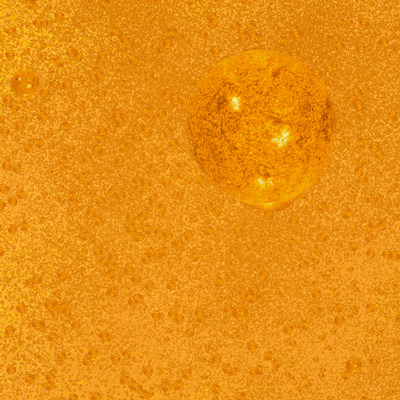
\includegraphics[width=0.35\textwidth]{olbers.png}}
\caption{Ілюстрація фотометричного ефекту в однорідному, ізотропному та статичному Всесвіті.}
\label{olbersIllust}
\end{figure}

Щоб пояснювати подібні явища, слід користуватися науковим методом. Спочатку задаться питання (``Чому небо вночі темне?''), потім, маючи якусь операцію, формуємо гіпотези. Далі проводяться експерименти, що перевіряють наші гіпотези, і результати експериментів аналізуються. Звідси робимо певні висновки, які дозволяють науковцям створити нові гіпотези, потім перевіряємо вже їх, і так далі. Саме так ми вдосконалюємо наше розуміння Всесвіту.

Ми зробили деякі припущення, але з цих припущень слідує модель Всесвіту, яка суперечить нашим спостереженням. Отже, деякі з наших гіпотез (припущень) не є вірними. Наприклад, видимий Всесвіт може бути скінченним, або ж кількість зірок у ньому скінченна. Можливо, він не є статичний, і це якимось чином відіграє роль в освітленні неба. Також слід розглянути варіант нерівноморного розподілу зірок: наприклад, їх нескінченно багато, проте вони вишукавні в ряди і ``ховаються'' одна за одною від Землі. \cite{relativityFAQ}

Тож перед нами стоїть питання: яку саме з цих гіпотез слід відкинути, і чим же її замінити? Кожне з цих припущень має колосальний ефект на наше розуміння космосу.

Сучасна астрофізика та космологія наводить пояснення цієї суперечності, тому в наш час це питання вважається вирішеним. Незважаючи на це, з оптометричним парадоксом варто ознайомитися, і для цього є декілька причин. 

По-перше, дослідивши історію цього парадоксу, можна отримати певне уявлення щодо розвитку астрофізики взагалі. Оптометричний парадокс був сформульований декілька століть тому, і взагалі цю проблему обговорювали ще у VII столітті. \cite{essential} Різні вчені у різних епохах висували свої пояснення цього парадоксу, і паралельно з еволюцією фізики в цілому, вдосконалювалися і пояснення.

По-друге, розглянувши сучасні пояснення парадоксу, можна трохи глибше зрозуміти сучасну космологію та астрофізику. Такі поняття, як червоний зсув, розширення Всесвіту та її скінченний вік, не надто інтуїтивні, і їх вплив на наше повсякденне життя не завжди є очевидним. Можна сказати, що це насправді чудово, що таке просте запитання, як ``Чому небо вдень світле, а вночі темне?'', дозволяє проілюстрювати ці поняття. \cite{introduction}

\textbf{Парадокс.}
На початку цього реферату ми навели деякі припущення щодо нашого Всесвіту. Давайте переконаємося, що з цих припущень дійсно мало би слідувати, що вночі небо світле. Нагадаємо наші припущення: Всесвіт статичний, вічний, і зорі рівномірно розподілені у нескінченному просторі. 

Освітленість від зорі з абсолютною світністю $L$ віддаленої на відстань $r$, дорівнюватиме $\dfrac{L}{4{\pi}r^2}$ (нехтуючи поглинанням світла).

\begin{figure}[ht]
\centering{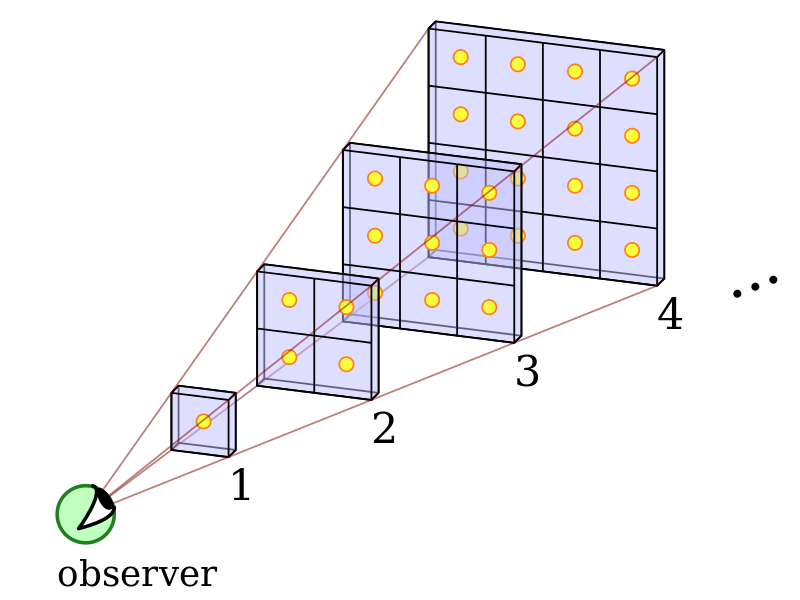
\includegraphics[width=0.4\textwidth]{observer.png}}
	\caption{Як спостерігач (observer) бачить ``оболонки'' неба}
\label{shells}
\end{figure}

Умовно розділимо Всесвіт на нескінченний набір ``оболонок'' навколо Землі, товщиною d. Якщо оболонки мають форму кулі, і якщо густина зір n постійна, то кількість зір, віддалених на відстань між $r$ і $r+dr$, дорівнює $4{\pi}nr^{2}dr$. Тоді густина загальної випроміненої енергії дорівнює:

\begin{equation}
\label{olbersProof}
\int\limits_{0}^{\infty}{\dfrac{L}{4{\pi}r^2} 4{\pi}nr^{2}dr} = Ln\int\limits_{0}^{\infty}dr
\end{equation}

Інтеграл у формулі (\ref{olbersProof}) розбіжний, тобто, густина енергії зоряного світла нескінченна.

Звичайно ж, ми знаємо, що зірки нерівномірно розподілені по Всесвіту: вони скупчуються у галактики, галактики - у групи та скупчення, а вони, в свою чергу, утворюють надскупчення. Проте наявність таких структур не дає нам вирішення парадоксу. Можна замінити слово ``зірка'' на ``галактика'', і міркування від цього не змінилася би. \cite{introduction} Винятком є ситуація, коли гіпотетичний Всесвіт має фрактальну структуру, її ми розглянемо пізніше.

\textbf{Історія.}
Парадокс Ольберса - один із випадків, коли певна ідея несе не ім'я того, хто вперше її сформулював. Найпершою згадкою проблеми про тепло, випромінене нескінченною кількістю зірок, вважається \textit{Topographia Christiana} грецького монаха Козьми Індик\'oплова (Індикоплевста), який у VI столітті нашої ери писав про кришталеве небо, що бере на себе все тепло Сонця, Місяця та безлічі зірок. Він вважав, що якби небо не було зроблено з кришталю, то воно би розплавилось або згоріло. \cite{essential} 

Пізніше це питання висунув Кеплер у 1610 році, який вважав, що цей парадокс є вагомим аргументом на підтримку моделі скінченного Всесвіту, або принаймні скінченної кількості зірок.У XVIII столітті більш розвинули цю ідею шфейцарський астроном Жан-Філіп Луї де Шезо та відомий англійський вчений Едмонд Галлей.

Дуже часто ідею цього парадоксу приписують німецькому астроному Генріху Ольберсу, який популяризував цей парадокс. Проте сучасні історики вважають, що Ольберс все ж не першим висунув це питання, і його здогадки щодо відповіді не мали наукової цінності.\cite{essential}

Шезо і Олбьерс спробували вирішити цей парадокс, припустивши, що світло далеких зір екранізується хмарами космічного пилу. Зараз же ми знаємо, що цим не можна пояснити парадокс, оскільки з законів термодинаміки відомо, що цей пил також би нагрівався та випромінював світло. Дійсно, пил може діяти як щит від радіації, і він може поглинути чи розсіяти певну кількість енергії. Проте аби достатньо захистити Землю від зоряного світла, необхідно було б мати стільки пилу у відкритому космосі, що воно би закривало і наше Сонце. Тому цю ідею серйозно сприймати не можна. \cite{relativityFAQ}

Вважається, що першу більш-менш правильну відповідь на цей парадокс надав Вільям Томсон, лорд Кельвін у статті 1901 року.

Цікавим є той факт, що аргумент Кельвіна були певною мірою передбачені відомим письменником Едгаром Алланом По у його есе \textit{Еврика} (1848), який він вважав за свій magnum opus. У творі згадується "відстань настільки велика, що жоден промінь ще не встиг до нас дійти". \cite{nyt}

\textbf{Пояснення.}
Ще раз звернемо увагу на аргументи Томсона та По. Дійсно, зараз нам відомо, що світло розповсюджується зі скінченною швидкістю. До того ж, вік Всесвіту вважається скінченним - приблизно 13,9 мільярдів років. Світло, випромінене об'єктами, що знаходяться на відстані більшій за 13,9 мільярдів світлових років, ще не мало достатньо часу, щоб його можна було спостерігати з Землі. Отже, видимий всесвіт має скінченний об'єм- з Землі до нас доходить світло лише зі скінченної кількості зірок. Ця кількість настільки мала, що якщо від Землі намалювати промінь у будь-якому напрямку, скоріше за все, він не досягне зірки.

Той факт, що вік Всесвіту скінченний, випливає з теорії Великого вибуху. Вона пояснює такі речі, як закон Габбла (чим далі від нас галактики, тим швидше вони від нас віддаляються),реліктове випромінювання та структуру Всесвіту у великих масштабах. \cite{introduction}

Ця сама теорія може створити і нову проблему, яка заважає поясненню фотометричного парадоксу. Вона стверджує, що в минулому, на початкових етапах формаування Всесвіту, небо було набагто світліше, особливо в еру рекомбінації (коли заряджені електрони і протони стають зв'язними, і внаслідок цього небо вперше стає прозорим). Температура Всесвіту на той момент була настільки великою, що її можна порівняти з температурою Сонця. Можна вважати, що більшість світлових променів з'явилося саме як релікт Великого вибуху, а не як випромінення з сучасних зірок.

Насправді ж, це не є для нас проблематичним. Теорія Великого вибуху містить в собі і вирішення проблеми, ніби-то створеної її самою. Оскільки Всесвіт розширюється, то енергія світла, яке випромінилось за часів Великого вибуху, зменшилась через червоний зсув. Цей ефект досить впливовий: високоенергічні хвилі, випромінені Великим вибухом, на цей момент є лише мікрохвилями; довжина хвилі збільшилася в 1100 разів. Тобто значення червоного зсуву, умовно кажучи, дорівнює $z = \dfrac{\lambda_{obsv}-\lambda_{emit}}{\lambda_{emit}} = 1099$. \cite{introduction} Зараз ці хвилі називають реліктовим випромінюванням, і їх можна побачити лише спеціальними пристроями, тобто вони не мають ніякого ефекту на видиість нічного неба.

Ефект червоного зсуву також діє на далекі зірки та квазари, які віддаляються від нас зі значною швидкістю через закон Габбла. Проте навіть найвіддаленіші такі об'єкти мають червоний зсув від 5 до 8,6. \cite{relativityFAQ}

Сучасні астрофізики вважають, що скінченний вік Всесвіту та червоний зсув - це два основних фактори, які пояснюють фотометричний парадокс. З точки зору математики, впливовішим серед цих факторів є саме вік Всесвіту. З іншого боку, деякі вчені стверджують, що якби Всесвіт не розширювався, то пояснити парадокс було би неможливо.

Уявимо собі статичний космос, у якому зірки розподілені рівномірно зі сталою густиною. Тоді температура Всесвіту би постійно підвищувалась. У певний момент часу ми би досягли стану рівноваги за температури 3000 К, тоді більшість простору займала би плазма, яка би почала поглинати фотони, і небо перестало би бути прозорим. При цьому густина енергії радіації досягла би $1,2 \times 10^{17} \dfrac{eV}{m^3}$, що в мільярди разів перевищує значення, яке ми спостерігаємо в реальності. \cite{introduction}

Насправді, навіть якби Всесвіт мав нескінченний вік, червоний зсув міг би пояснити цей парадокс. Для цього розглянемо теорію статичного Всесвіту.

У теорії статичного Всесвіту, він має скінченний вік, і в той же час він постійно розширюється. Густина матерії у ній залишається сталою через постійне створення нової матерії, тобто принцип ізотропії та однорідності зберігається.

Хоча ця теорія й мала деяких прихильників на початку XIX століття, зараз більшість космологів та астрофізиків не сприймають її серйозно. Сучасні експерименти і дослідження вказують саме на космологію Великого вибуху, і що вік Всесвіту таки скінченний. \cite{twoTheories}

Незважаючи на це, спробуємо пояснити фотометричний парадокс так, як це робили вчені 100 років тому. З закону Планка матимемо таку густину енергії для отриманих хвиль:

\begin{equation}
\label{steadyStateEnergy}
\dfrac{U}{V} = \dfrac{8\pi^5(kT)^4}{15(hc)^3}
\end{equation}

Для температури 2,7К матимемо густину енергії $40 \dfrac{fJ}{m^3}$ або $4,5 \times 10^{-31} \dfrac{kg}{m^3}$, в той час як для температури 6000К поверхні Сонця матимемо $1 \dfrac{J}{m^3}$ або $1,1 \times 10^{-17} \dfrac{kg}{m^3}$. Проте повна радіація, випромінена небесним тілом, не може перевищувати атомній енергіїі ізотопів, які містяться у тілі. Знаючи густину видимого Всесвіту ($4,6 \times 10^{-28} \dfrac{kg}{m^3}$) та розповсюдженість хімічних елементів, маємо загальну густину енергії $82 \dfrac{fJ}{m^3}$ і температуру 3,2К. Цікаво те, що це значення достатньо близьке до суми виміряних значень густини енергії мікрохвильового та нейтронного реліктових випромінювань. \cite{twoTheories}

Маючи ці знання, ми можемо детальніше розглянути ще один період розвитку астрофізики - на цей раз, більш сучасний. Після того, як на початку ХІХ століття був відкритий закон Габбла (який, до речі, зараз називають законом Габбла-Леметра. \cite{hubbleLemaitre}), але до того, як розвинулася теорія Великого вибуху, фотометричний парадокс вважали доказом спеціальної теорії відносноті. Аби позбутися ``зайвого світла'', знадобилося поняття червоного зсуву. \cite{relativityFAQ}

\textbf{Інші фактори.}
Ми розглянули два основні фактори, які пояснюють наш парадокс: скінченний вік Всесвіту та червоний зсув. Розглянемо також деякі інші пояснення, які, можливо, теж відіграють певну роль.

Одним із аргументів, запропонованих для пояснення фотометричного парадоксу, є скінченний вік зірок. Зірки не живуть вічно, і не віддають нескінченну кількість енергії, тобто вплив кожної зірки на освітлення нічного неба обмежений. Цю ідею висунув раніше згаданий Едгар Аллан По, і пов'язану з цим теорію запропонував Жан-Філіп де Шезо. Зараз же нам відомо, що зірки постійно як і вмирають, так і народжуються. За умови, що загальна густина зірок залишається сталою, у будь-якому напрямку від Землі матимемо нескінченний набір зірок, і їх загальний вплив буде нескінченним. Це справджується як і у ``вічному'' Всесвіті, так і для Всесвіту зі скінченним віком.

Є ще одне пояснення парадоксу, яке не спирається на теорію Великого вибуху - це фрактальний розподіл зірок. Цю ідею вперше висунув Карл Шарьє у 1908 році, і пізніше її запропонував Бенуа Мандельброт, незалежно від Шарьє, у 1974 році. Вони обидва постулювали, що якщо матерія у Всесвіті розподілена в ієрархічній фрактальній космології, то не обов'язково приймати умови теорії Великого вибуху, аби пояснити фотометричний парадокс. Ця ідея не суперечить існуванню вибуху, лише стверджує, що середня густина будь-якого регіону зменшується, якщо розглядати більші регіони. \cite{introduction}

Якщо наш Всесвіт дійсно так розподілений, то світність, отриману з зірок, можна математично зобразити так:

\begin{equation}
\label{fractalLuma}
	\int\limits_{r_{0}}^{\infty}L(r)N(r)dr
\end{equation}

де $r_{0}$ - відстань від Землі до найближчої зірки, $r$ - змінна, що виражає відстань від Землі, $L(r)$ - середня світність, отримана з зірки на відстані $r$, $N(r)$ - кількість зірок на відстані $r$. \cite{introduction}

Мажмо функцію світності, отриманої з певної відстані від Землі $L(r)N(r)$, від якої залежить, чи буде небо нескінченно освітленим, чи ні. Якщо $L(r)N(r)$ лінійно пропорційний до $r^a$, то інтеграл буде розбіжним для $a{\geq}-1$, або ж матиме скінченне значення для $a<-1$. Припустимо, що при віддаленні в $n$ разів, кількість отриманих світлових променів зменшується в $n^2$ рази, тобто $L(r)$ пропорційна до $r^{-2}$. Тоді щоб вирішити парадокс Ольберса-Шезо, необхідно, щоб $N(r)$ було пропорційне до $r^b$, де $b<1$. Якщо $b=1$, кількість зірок, розташованих на певній відстані, буде пропорційною до цієї відстані. Тобто загальна кількість зірок дорівнює $r^2$. Можна сказати, що це є рівномірний розподіл зірок, або що йому відповідає фрактальна розмірність 2. Щоб отримана світність була скінченною, фрактальна розмірність повинна бути менша, за 2.

Хоча, з чисто теоретичної точки зору, вчені не заперечують таке пояснення \cite{relativityFAQ}, більшість із них приймають так званий космологічний принцип. Тобто вважається, що Всесвіт однорідний (незалежність від місця спостережень) та ізотропний (незалежність від напрямку). Цей принцип суперечить фрактальній космології, яка потребує анізотропію. \cite{introduction}

\textbf{Висновки.} Питання ``Чому небо вночі темне?'' виявилося дійсно цікавим. Ми розглянули досить багато різних пояснень, починаючи від міркувань давніх греків і закінчуючи сучасними теоріями про Всесвіт. Всі ці пояснення ілюструють певну модель Всесвіту, і ми бачимо, як ця модель вдосконалювалася з часом.

Взагалі, можна сказати, що це чудова ілюстрація наукового методу. Вчені, намагаючись пояснити певні явища, створюють гіпотези, потім експериментальним чином перевіряють ці гіпотези. Якщо спостерігається неочікуваний результат, то створюються нові гіпотези, а старі відкидаються - рано чи піздно ми отримуємо більш точну модель Всесвіту. Все це починається зі сформульованого питання. Ми бачимо, що питання фотометричного парадоксу штовхало вчених до висування нових ідей, отже воно є важливою частиною історії фізики.

\begin{thebibliography}{9}
{\small
\bibitem{relativityFAQ} Chase~S.\,I. 2004, Relativity FAQ about Olbers's paradox, http://math.ucr.edu/home/baez/physics/Relativity/GR/olbers.html
\bibitem{nyt} Overbye~D., 2015, The Flip Side of Optimism About Life on Other Planets, The New York Times
\bibitem{dictionary} Климишин~І.\,А., Корсунь~А.\,О. 2003, Астрономічний енциклопедичний словник
\bibitem{essential} Heyller\,~Markus,~ed. 2008, The Scientific Revolution: The Essential Readings
\bibitem{hubbleLemaitre} International Astronomical Union 2018, "IAU members vote to recommend renaming the Hubble law as the Hubble–Lemaître law". Прес-реліз.
\bibitem{introduction} Willaman~V.\,M., 2006, Introduction to Cosmology and Olbers' Paradox, http://personal.psu.edu/wnb3/psiwa-2006-cosmology/notes-all.pdf
\bibitem{twoTheories} Helge~K. 1999, Cosmology and Controversy: The Historical Development of Two Theories of the Universe
}
\end{thebibliography}

\end{document}
